% This is samplepaper.tex, a sample chapter demonstrating the
% LLNCS macro package for Springer Computer Science proceedings;
% Version 2.20 of 2017/10/04
%
\documentclass[runningheads]{llncs}
%
%\usepackage{fullpage}
%\usepackage{setspace}
%\onehalfspacing
\usepackage{listings}
\usepackage{graphicx}
% Used for displaying a sample figure. If possible, figure files should
% be included in EPS format.
\usepackage{makecell}
\renewcommand\theadfont{\bfseries}
%
% If you use the hyperref package, please uncomment the following line
% to display URLs in blue roman font according to Springer's eBook style:
%\renewcommand\UrlFont{\color{blue}\rmfamily}

\begin{document}
%
\title{BLAST: Block Applications for Things}
%
%\titlerunning{Abbreviated paper title}
% If the paper title is too long for the running head, you can set
% an abbreviated paper title here
%
\author{Michael Freund\inst{1}\orcidID{0000-0003-1601-9331} \and
Thomas Wehr\inst{1}\orcidID{0000-0002-0678-5019} \and
Andreas Harth\inst{1,2}\orcidID{0000-0002-0702-510X}}
%
\authorrunning{M. Freund et al.}
% First names are abbreviated in the running head.
% If there are more than two authors, 'et al.' is used.
%
\institute{Fraunhofer Institute for Integrated Circuits IIS, Nürnberg, Germany 
\email{firstname.lastname@iis.fraunhofer.de}\\
\and
Friedrich–Alexander University Erlangen-Nürnberg, Nürnberg, Germany}
%
\maketitle              % typeset the header of the contribution
%
\begin{abstract}
  We introduce a block-based visual programming language called BLAST to write programs involving connected devices with a Web of Things abstraction.
  We developed an editor and an execution environment for BLAST programs that runs in a web browser.
  We demonstrate that BLAST can be used to create programs that interact with a variety of devices.
  In particular we show the use of connected devices in a geofencing scenario.
\keywords{Block-based Programming \and Web of Things.}
\end{abstract}
%
%
%
\setcounter{footnote}{0}
\section{Introduction}
Connected devices form the basis for a wide variety of applications in industry settings, such as condition monitoring, energy consumption analysis, simulation and optimisation~\cite{CIMINO2019103130}.
%Given the multitude of protocols for interacting with such devices, application development is difficult.
The Web of Things (WoT)\footnote{\url{https://www.w3.org/WoT/}} aims at providing a set of standardised technologies to help simplify the creating of applications involving connected devices.
At the same time, casual users should be able to quickly program applications involving connected devices.
The programming languages currently in use for accessing devices are primarily text-based and are difficult to access for casual users.
One possible approach to improve accessibility and simplify the creation of computer programs is the visual programming paradigm.

Visual programming does not require the user to enter any text; instead, programs are based on graphical elements like blocks, graphs, tables or diagrams.
Programs are created by arranging predefined blocks with images or text are arranged into programs via a drag-and-drop interface.
Blocks can be geometrically aligned with other compatible blocks, like in a jigsaw puzzle, to form complex programs.
Since blocks can only be arranged in the correct way, no syntax errors can occur~\cite{10.11453341221}~\cite{maloney2010scratch}~\cite{10.1145/1089733.1089734}.

The created block programs can be translated into any predefined programming language, resulting in a normal source code. 
The block-based approach can be used not only for learning programming concepts, but also for more complex problems.
For example, block languages have been successfully used in programming industrial robots~\cite{8120406}~\cite{ghazal2016framework}~\cite{tomlein2017visual} or executing SPARQL queries~\cite{7369012}, both areas which normally require advanced programming skills.

We present BLAST, a visual programming environment that works with devices following the Web of Things interface.
BLAST programs can be created in a web browser, based on Google's Blockly\footnote{\url{https://developers.google.com/blockly/}}, a JavaScript library for creating block-based languages and editors.
BLAST programs can be translated to JavaScript and executed in the web browser.
BLAST implements the Web of Things abstraction to devices with Bluetooth Low Energy (BLE) and USB Human Interface Devices (HID) interface via APIs of modern web browsers.

The currently best known tool for programming IoT devices using visual programming is Node-RED\footnote{\url{https://nodered.org/}}.
In contrast to BLAST, which focuses on control flow constructs, Node-RED's programming paradigm is based on dataflows.
The use cases in industrial settings we envision for BLAST involve mostly control flow, and in such scenarios a dataflow abstraction can lead to programs that are difficult to understand and maintain.
%The nodes in these graphs are black box processes, created by the developers, that can be connected to each other by the end user.
%The block-based approach utilized by BLAST provides more flexibility as its blocks are a lot more fine grained.
%BLAST is a programming language with a

Another system similiar to BLAST is Punya~\cite{patton2021punya}, an Android app development system based on the MIT App Inventor\footnote{\url{https://appinventor.mit.edu/}}.
Like BLAST, Punya offers a block-based programming environment able to run SPARQL queries and include online services.
Punya focuses on creating applications for Android devices and communicates with the mobile phones's internal hardware, in addition to working as a LDP-CoAP client to publish and access data on CoAP servers.
BLAST programs, on the other hand, run in modern web browsers and support devices based on a Web of Things abstraction.

In the following we first introduce the BLAST language using a geofencing scenario, next describe the browser-based editor and execution environment for BLAST programs and then conclude.

\section{BLAST Language}

When choosing the vocabulary for our block-based language BLAST, we decided on a mixture of natural language and computer language~\cite{8120404}.
In BLAST, the blocks are arranged into readable sentences, as in a natural language, but the blocks also contain a few technical programming terms, such as ''repeat while true'' instead of ''forever''.

The BLAST language includes standard elements from other programming languages such as loops, functions, and variables.
In addition, the BLAST language provides blocks related to interacting with WoT devices.
These WoT-related blocks can be grouped under the three interaction affordances Properties (that can be read and written), Actions (that can be invoked), and Events (that can be observed).
Further, the BLAST language includes blocks to send HTTP requests with arbitrary headers, request method and request body.
Using HTTP requests, one can load RDF graphs from a URI and execute SPARQL queries, which allows for the interaction with Read-Write Linked Data APIs or other REST APIs.
Finally, if the available blocks are not sufficient to implement a desired functionality, there is a block in which native JavaScript code can be entered, and thus almost everything that is possible in JavaScript is also possible in BLAST.

For an example for a BLAST program see figure \ref{fig1}.
The program involves a LED light with a BLE interface and a small battery-powered BLE beacon.
The BLE controller (the ``BLE central'') is implicitly used when reading the signal-strength property.
The functionality of these devices (``Things'') can be accessed via reading and writing properties.
The LED light, for example, has a property ``colour'' that can be written.
To enable an event abstraction, the program includes a block that defines a state with a condition on the signal strength of the BLE beacon.
On entering or exiting the defined state, the event blocks, which can contain arbitrary blocks, are triggered.

\begin{figure}
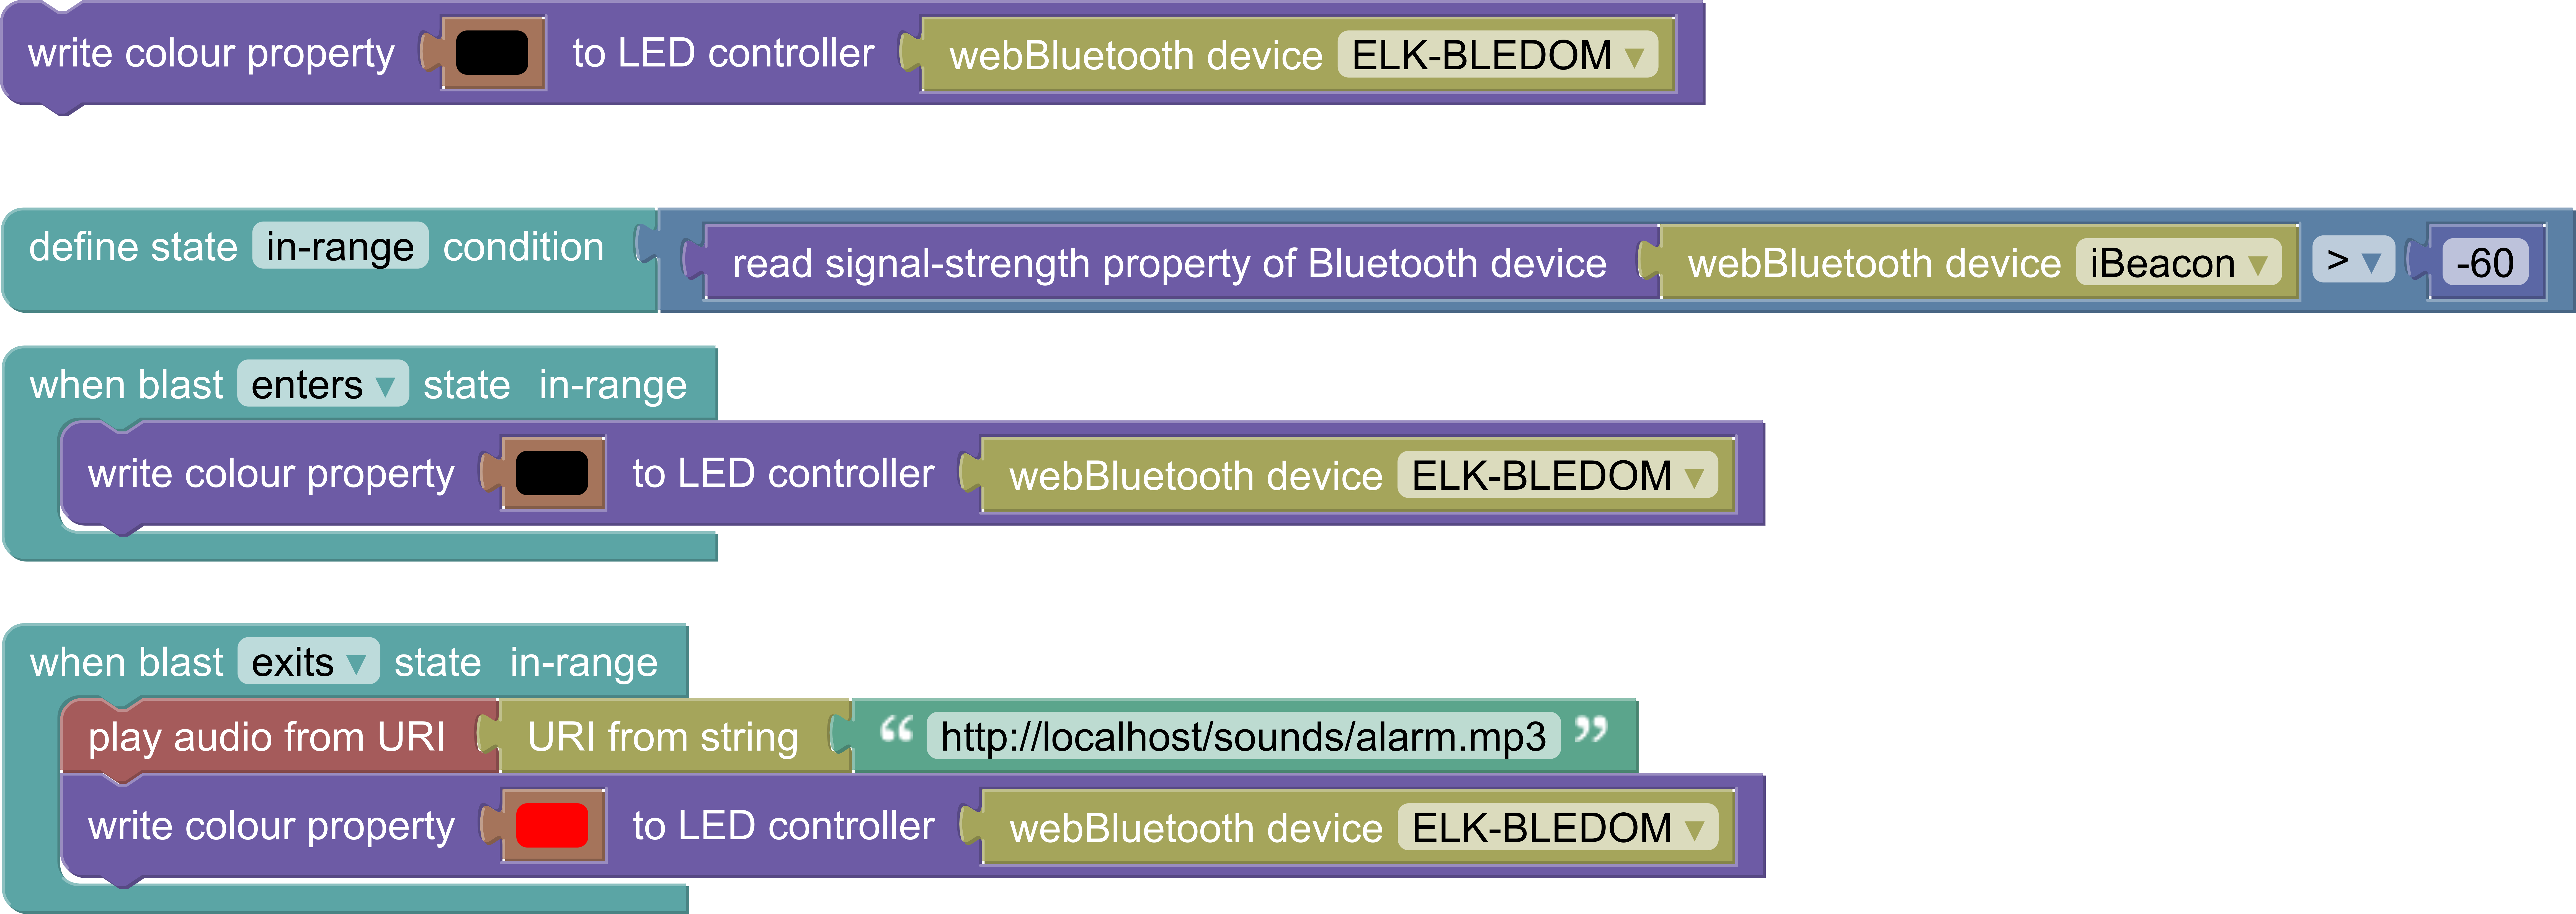
\includegraphics[width=\textwidth]{screenshot 3.png}%im Ordner sind noch 2 alternative Screenshots
\caption{Example BLAST program that implements a geofencing scenario: when the beacon gets close, the light is turned off; when the beacon leaves the close range, the light is turned red.} \label{fig1}
\end{figure}

\section{BLAST Editor and Execution Environment}

We have implemented an editor and an execution environment for BLAST programs that runs in a modern web browser.


uses Web Bluetooth to communicate with IoT devices, custom control and command blocks, and generates JavaScript code that can be used by any JavaScript interpreter.
To interact with the IoT devices, BLAST requires custom drivers for each device, which represent an extended form of the WoT TD % Beides noch nicht definiert
and contain the metadata and interaction affordances as well as the JavaScript code needed for communication.

Supported Devices and Services

To demonstrate how BLAST can interact with WoT devices, we provide a Web of Things abstraction for devices communicating with Bluetooth Low Energy and USB Human Interface Devices (HID).
We also provide access to online APIs related to speech input and output and services like playing audio from a URI or invoking SPARQL queries on an online ressource.

\begin{center}
  \begin{tabular}{|c|c|c|}
  \hline
  \thead{Device} & \thead{Communication} & \thead{WoT interactions} \\
  \hline
  Eddystone Devices & BLE GATT & read/write Eddystone properties \\
  \hline
  HuskyLens\footnote{https://wiki.dfrobot.com/HUSKYLENS\_V1.0\_SKU\_SEN0305\_SEN0336} & BLE GATT & read sensor properties, invoke forget action \\
  \hline
  RGB LED Controller\footnote{https://aliexpress.com/item/4000208329326.html} & BLE GATT & write color properties \\
  \hline
  RuuviTag\footnote{https://ruuvi.com/ruuvitag/} & BLE GAP & \makecell{read sensor properties, read battery property, \\
  read/write txPower property, \\
  read movement counter propert,y \\
  read measurement sequence counter property} \\
  \hline
  StreamDeck\footnote{https://www.streamdeck.com/} & USB HID & \makecell{write display properties, \\ subscribe to button push events} \\
  \hline
  Tulogic BlinkStick\footnote{https://www.blinkstick.com/} & USB HID & write color properties \\ 
  \hline
  Nintendo JoyCon\footnote{https://www.nintendo.com/switch/tech-specs/\#joycon-section} & USB HID \& BLE GATT & \makecell{read sensor properties,\\ subscribe to button push events} \\
  \hline
  Xiaomi Thermometer\footnote{https://xiaomipedia.com/en/p/xiaomi-electronic-thermometer-and-hygrometer/} & BLE GAP & read sensor properties \\
  \hline
  \end{tabular}

  \begin{tabular}{|c|c|}
  \hline
  \thead{Service} & \thead{WoT interactions} \\
  \hline
  Camera & invoke capture image action \\
  \hline
  Audio & invoke play audio action \\
  \hline
  WebSpeech API & invoke text to speech action, invoke speech to text action \\
  \hline
  HTTP Requests & invoke send HTTP request action \\
  \hline
  SPARQL Query & invoke execute SPARQL query action \\
  \hline
  SOLID & invoke upload to solid container action \\
  \hline
  \end{tabular}
\end{center}

\section{Conclusion}

Our block-based language simplifies the interaction with IoT devices, digital twins or other web resources without the need for a deeper understanding of different programming languages or network protocols such as Bluetooth or HTTP.
As IoT devices become increasingly relevant in the industrial environment, investigating how the interaction between humans and the IoT devices can be seamlessly implemented.
We have explored the use of block-based programming environment to interact with devices.
We have also implemented a more complex logistics scenario involving an automated picking line to prepare orders.

We are currently working on a way to execute the created BLAST program independently of browsers.
To this end, we are developing an execution environment that can load BLAST programs, convert them to JavaScript, and execute them as a server.
%In the future, it would enrich BLAST if there was a way to consume WoT TDs and derive interaction possibilities, which would allow BLAST to interact with any WoT device.
%@@@Web Bluetooth has certain restrictions (security, reading RSSI), server should not have these restrictions.

%
% ---- Bibliography ----
%
% BibTeX users should specify bibliography style 'splncs04'.
% References will then be sorted and formatted in the correct style.
%
\bibliographystyle{splncs04}
\bibliography{references}
%

\end{document}
